%\documentclass[12pt]{journal}
\documentclass[sigplan,nonacm]{acmart}
\usepackage[english]{babel}
\usepackage[utf8x]{inputenc}

%\usepackage{amsmath,amssymb,amsthm}
\usepackage{tcolorbox}
%\newtcbox{\inlinecode}{on line, boxrule=0pt, boxsep=0pt, top=2pt, left=2pt, bottom=2pt, right=2pt, colback=gray!15, colframe=white, fontupper={\ttfamily \footnotesize}}

%\usepackage{enumerate}
\usepackage{graphicx}
\usepackage{booktabs,tabularx}
\usepackage{pgf,tikz,tikz-3dplot}
\usepackage{caption}
\usepackage{float}
\tikzset{%
	no/.style={draw, rounded corners, thick, fill=gray!40},
	arrow/.style={thick,->,>=stealth',shorten >=1pt}}


\begin{document}
\title{}

\author{Brandon Hosley}
\orcid{0000-0002-2152-8192}
%\authornotemark[1]
%\authornote{text}
\email{brandon.hosley.1@us.af.mil}
\affiliation{%
	\institution{Air Force Institute of Technology}
	\streetaddress{1751 11th St.}
	\city{Wright-Patterson Air Force Base}
	\state{Ohio}
	\country{USA}
	\postcode{45433}
}

\begin{abstract}
	An exploratory analysis of possible mechanisms for producing
	unsupervised semi-salient image segmentation, resulting in
	usable image sets for training models aimed at other computer vision tasks.
\end{abstract}

\received{\today}
\maketitle

\section{Introduction}
\subsection{Overview}

This proposal will outline the research performed to fulfill the requirements of 
CSCE 632 - Statistical Machine Learning; 
to demonstrate competency of the topics presented in the course.
In this proposal we will outline the background and motivation behind the project,
briefly discussing the larger problem to be solved, and how this smaller project
is intended to fit into that objective.

An outline of the data science trajectory, data source, and data preparation that
will be used in this project.
To conclude this proposal we will discuss what the intended contribution of this project
to the body of Computer Vision writ large will be.


\subsection{Motivation}

The CMP facade dataset \cite{tylecek2013}
is a collection of images of building facades which have been rectified and
have a number of distinct architectural features manually labeled.
One use of this dataset is shown in \cite{isola2018}
where the authors use the labeled building data to train a generative adversarial network
to produce realistic, synthetic images of building facades.
Other potential applications of this type of model will be left to the imagination of the reader.

\begin{figure}
	\centering
	\includegraphics[width=0.9\linewidth]{"Screenshot 2023-04-21 at 9.38.01 PM"}
	\caption{Building with corresponding architectural feature masks.}
	\label{fig:buildings}
\end{figure}

The objective of this project is to attempt to produce similar feature labeling but
via an application of unsupervised salient object detection.
Or to identify groups of three dimensional primitives using a histogram of gradients technique.

Additionally, due to external constraints this is to be done without using any sort of neural network.


\section{Data Science Trajectory}

The pipeline for this project will consist of data value exploration
followed by data understanding, data preparation, modeling, and evaluation;
then repeat from data preparation until a usable model is achieved.

\begin{figure}
	\centering
	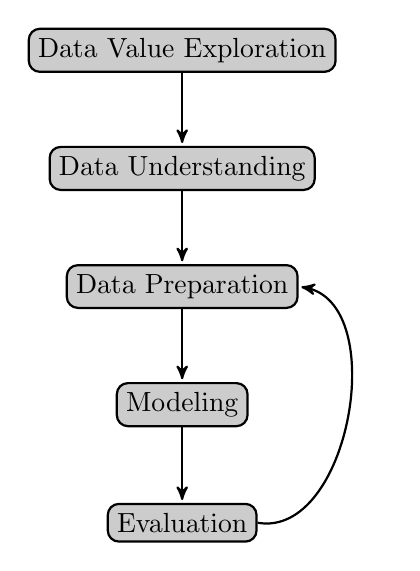
\begin{tikzpicture}[node distance=1.5cm]		
		\node[no] (DVE) {Data Value Exploration};
		\node[no] (DU) [below of=DVE] {Data Understanding};
		\node[no] (DP) [below of=DU] {Data Preparation};
		\node[no] (MO) [below of=DP] {Modeling};
		\node[no] (EV) [below of=MO] {Evaluation};
		
		\path[arrow] (DVE) 	edge []  node [] 	{} (DU);
		\path[arrow] (DU) 	edge []  node [] 	{} (DP);
		\path[arrow] (DP) 	edge []  node [] 	{} (MO);
		\path[arrow] (MO) 	edge []  node [] 	{} (EV);
		\path[arrow] (EV) 	edge [bend right, out=-90, in=-90]  node [] 	{} (DP);
		%\path (FS)  	edge []  node [below] 	{\(0.7\)} (FMC);
		%\path (BS3) 	edge [bend left, in=120]  node [below] 	{\(0.8\)} (FMC);
		%
		%\path (FMC) 	edge [bend left]  node [above] 	{\(0.2\)} (FS);
		%\path (BS3) 	edge []  node [below left] 	{\(0.2\)} (FS);
		%
		%\path  (FS) 		edge []  node [above left] 	{\(0.3\)} (BS1);
		%\path  (BS1) 	edge [bend left=25]  node [above right] 	{\(1.0\)} (BS2);
		%\path  (BS2) 	edge [bend left=25]  node [below right] 	{\(1.0\)} (BS3);
	\end{tikzpicture}
	\caption{Data Science Trajectory.}
	\label{DTMC}
\end{figure}

\section{Data Acquisition and Preparation}

The dataset to be used is comprised of approximately 20GB of images of consumer motor vehicles.
It has generously been made available by \cite{yang2015}
and has several aspects that we expect will be very useful towards our goals.

Additionally, this data has been sanitized and will be ready for use immediately.
The sizes of images are consistent among the types of image groups within the dataset.
Conveniently, this set includes a set of labeled features that may be useful in 
attempting to identify if produced groups of primitives can be correlated with
features typically recognized by humans.

\section{Data Exploration}

The \cite{yang2015} dataset contains 136,727 images of motor vehicle bodies with 
several labels attached to the images; some of which will be immediately useful.
Each vehicle has a hierarchical set of labels constituting the make, model, and year.
Specifically, the set includes 161 makes and 1,687 models spread approximately across
the years 2005 to 2015. The vehicles are further divided by class of body-type; 
MPV, SUV, hatchback, sedan, minibus, fastback, estate, pickup, sports, crossover, convertible, and hardtop convertible.
There are five different points of view; front, rear, side, side-front, side-rear.

\begin{figure}
	\centering
	\includegraphics[width=0.9\linewidth]{"Screenshot 2023-04-21 at 9.46.15 PM"}
	\caption{Perspectives of Vehicles.}
	\label{fig:car_perspectives}
\end{figure}

The \cite{yang2015} dataset also contains 27,618 images capturing parts
of the vehicles such as headlight, taillight, fog light, and air intake; which will be used and
console, steering wheel, dashboard, and gear lever; which will not be used.

\begin{figure}
	\centering
	\includegraphics[width=0.9\linewidth]{"Screenshot 2023-04-21 at 9.46.00 PM"}
	\caption{Motor vehicle part features}
	\label{fig:screenshot-2023-04-21-at-9}
\end{figure}


The final class of images are surveillance-nature data containing 50,000 images capturing
the vehicle front view from an elevated perspective, which will not be used for this project.

\section{Expected Contributions}

Over the last decade computer vision has improved at an incredible pace.
Particularly within the areas of object detection, classification, and identification.
The flexibility of various models to perform these tasks has proven to be very effective.

One of the tasks that remains difficult for computers to do is to infer traits about unseen portions
of objects that it is built to identify.
Similarly, there are limits on the effectiveness of models when it comes to significant
changes in perspective when compared to the training data provided.
This problem will be significantly exacerbated when the training data set has few samples
or the samples all occur from a narrow perspective.

With this project we wish to increase the flexibility of performing identification of objects in spite
of an extremely small reference set.
Additionally, we hope that the deconstruction of objects in the manner presented in this paper will allow
us to create a larger synthetic training set using information about features extracted from minority
samples and inference based on information provided by a larger set so that other training tasks can be performed.
Among these tasks we intend to evaluate the implementation of lighter and smaller object identification models, 
and improving the reconstruction of three dimensional models of the objects depicted in limited view. 

%\section{Publication Venues}
%\section{Additional Methods}
\bibliographystyle{ACM-Reference-Format}
\bibliography{proposal}

\end{document}